\documentclass[12pt,a4paper]{article}
\usepackage[utf8]{inputenc}
\usepackage{amsmath}
\usepackage{amsfonts}
\usepackage{amssymb}
\usepackage{tikz}
\usepackage{amsmath}
\usepackage{amssymb}
\usepackage{pgfplots}
\usepackage{nccmath}
\usepackage{mathtools}
\usepackage{pgfplots}
\usepackage{mathtools,amssymb}
\usepackage{tikz}
\usepackage{xcolor}
\pgfplotsset{compat = newest}
\author{Chris Camano: ccamano@sfsu.edu}
\title{MATH301 HW 1 }
\date{1/29/2022}
% Margins
\topmargin=-0.45in
\evensidemargin=0in
\oddsidemargin=0in
\textwidth=6.5in
\textheight=9.0in
\headsep=0.25in


\begin{document}
\maketitle
\section{Section 1.1: problems A6,B22,B24,C34}\\
\textbf{A6: +++}\\
\begin{align*}
  \text{Let} A = \{x \in \mathbb{R} | x^2=9\}\\
  \sqrt{9}=-3,3 \therefore\\ A= \{-3,3\} \text{ as } \nexists x \in \mathbb{R} | x^2=9, x \notin{ 3,-3}
\end{align*}
This problem was very straight forward to me. In english: The set of numbers that satisfy the criterion $x^2=9$ is equal to $\{3,-3\}$ as there does not exist a real number such that $x^2=9$ besides 3 and -3.\\\\
\textbf{B22: +++}\\
\begin{align*}
  A=\{3,6,11,18,27,38,...\} =\\
  A=\{n^2+2:n \in \mathbb{N}\}\\\\
  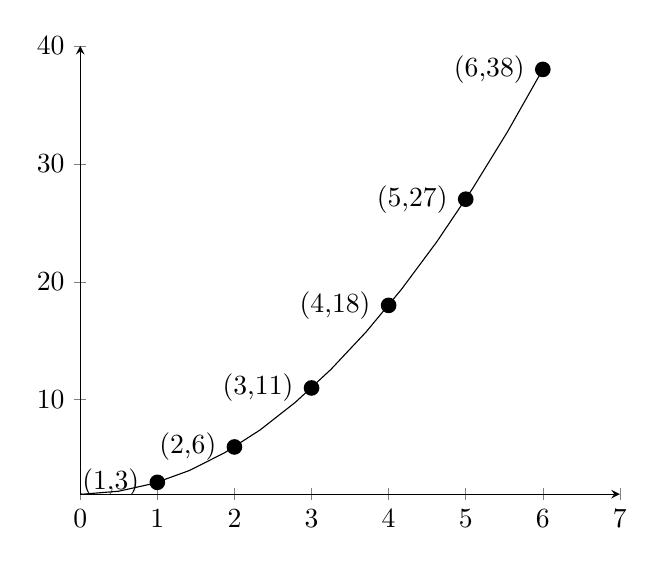
\begin{tikzpicture}
    \begin{axis}[axis y line=middle,axis x line=bottom, xmin=0,xmax=7,ymax=40, domain = -5:6]
        \addplot[mark=none] {x^2+2};
        \node[label={180:{(1,3)}},circle,fill,inner sep=2pt] at (axis cs:1,3) {};
        \node[label={180:{(2,6)}},circle,fill,inner sep=2pt] at (axis cs:2,6) {};
        \node[label={180:{(3,11)}},circle,fill,inner sep=2pt] at (axis cs:3,11) {};
        \node[label={180:{(4,18)}},circle,fill,inner sep=2pt] at (axis cs:4,18) {};
        \node[label={180:{(5,27)}},circle,fill,inner sep=2pt] at (axis cs:5,27) {};
        \node[label={180:{(6,38)}},circle,fill,inner sep=2pt] at (axis cs:6,38) {};
    \end{axis}
\end{tikzpicture}
\end{align*}
The set associated with this problem can be described by the function $f(n)=n^2+2$. I arrived at this point after researching arithmetic seaquences to no avail and finally resorting to plotting the points in the set alongside their index which helped me observe the quadratic pattern. Additionally I considered describing the set for all integers before realizing that the counting starts at index 1 and thus should be $\mathbb{N}$.Side note this was a really hard tikz picture to make ! who knew plotting points along a function was so hard.
\\\\
\textbf{B24: +++}\\
This question was not very hard for me and was as simple as bounding the integers from -4 to 2.
\begin{align*}
  A=\{-4,-3,-2,-1,0,1,2\}=\\
  A=\{x \in \mathbb{Z}|-4 \leq x \leq 2\}
\end{align*}
\textbf{C34:+++}\\
This question was straight forward and required me to list all numbers with absolute value less than ten within $\mathbb{N}$ before calculating cardinality.
\begin{align*}
  \text{Let } A= |\{x \in \mathbb{N} | |x| < 10\}|\\
  A=\{1,2,3,4,5,6,7,8,9\}\\
  |A|=9
\end{align*}

\section{Section 1.2: B12,B14}
\textbf{B12:+++}\\
See attached photo for work (still learning tikz) . This figure is a box with corners (-1,1),(-1,2),(1,1),(1,2) in $\mathbb{R}^2$.
\\\\
\textbf{B14:+++}\\
This problem required me to identify that the question was finding a product of an interval with a set and thus should have a restricted output. This means that only the ordered pairs with y components from the set $\{1,1.5,2\}$ should be considered.
\\\\
\section{Section 1.3: C14,C15}\\
\textbf{C14:+++}\\
Describe if the following statement is true or false:
\[
  \mathbb{R}^2 \subseteq \mathbb{R}^3
\]
\newcommand{\rtwo}{\mathbb{R}^2}
\newcommand{\rthree}{\mathbb{R}^3}

}
I believe that this statement is \textbf{false}  for the following reasons. Firstly setting the z component of $\mathbb{R}^3$ to 0 yields all of $\mathbb{R}^2$ while this is a tempting description that creates the illusion of $\mathbb{R}^2$ existing within $\rthree$ the fact is that you can choose any fixed point to construct a plane in three dimensions. So this is not truly a subset or rather subspace. Instead it is a space that is similar in character to $\rtwo$ but not the same. Since the selection of which plane you want to put in $\rthree$ is arbitrary there is no way to place $\rtwo$ within $\rthree$ in a way that validates the claim that it is a subspace. This problem is tricky to think about, but I am sure that it is the fact that the two dimensional plane can be placed in infinite configurations within $\rthree$ that makes it not a subspace.
\\\\
\textbf{C15:+++ }\\
Is the following true or false:
\[
  \{(x,y)\in \rtwo |x-1=0\}\subseteq \{(x,y) \in \rtwo|x^2-x=0\}
\]
I belive that this statement is \textbf{true} as the criterion x-1=0 has one solution when expressed as a function at x=1 the solution of the equation. Likewise $x^2-x=0$ has solutions when plotted including x=1 as:
\begin{align*}
  x^2-x=0\\
  x(x-1)=0\\
x=0,x=1
\end{align*}
Thus the set of all numbers of the form $(1,y),y\in \rtwo$ is contained as a subset of $\{(x,y) \in \rtwo|x^2-x=0\}$ as $\{(x,y) \in \rtwo|x^2-x=0\}$= all numbers of the form $\{(0,y),(1,y)\} y\in \rtwo$
\\
I am very confident with this answer and have verified my results graphically.
\\
\section{1.4: A2,A7}
\textbf{A2:+++}\\
Write the following sets by listing their elements
\begin{align*}
  \mathscr{P}(\{1,2,3,4\})=\{\emptyset,\{1\},\{2\},\{3\},\{4\},\{1,2\},\{1,3\},\{1,4\},\{3,4\},\{2,4\},\\
  \{2,3\},\{1,2,3\},\{2,3,4\},\{1,2,4\},\{1,2,3,4\},\{1,3,4\}\}
\end{align*}
This problem was tricky due to the fact that I had to consider all possible combinations of the sets. Luckily this checks out as there are 16 subsets which follows the rules presented in the book such that there exists $2^n$ subsets.
\\

\textbf{A7:+++}\\
Write the following sets by listing their elements:
\[
  P(\{a,b\})xP(\{0,1\})
\]

\begin{align*}
  P(\{a,b\})\text{ x }P(\{0,1\})=
  \{\emptyset,\{a\},\{b\},\{a,b\}\}x\{\emptyset,\{0\},\{1\},\{0,1\}\}=\\
\end{align*}
\begin{align*}
  \{(\emptyset,\emptyset),(\emptyset,\{0\}),(\emptyset,\{1\}),(\emptyset,\{0,1\}),\\(\{a\},\emptyset),(\{a\},\{0\}),(\{a\},\{1\}),(\{a\},\{0,1\}),\\(\{b\},\emptyset),(\{b\},\{0\}),(\{b\},\{1\}),(\{b\},\{0,1\}),\\(\{a,b\},\emptyset),(\{a,b\},\{0\}),(\{a,b\},\{1\}),(\{a,b\},\{0,1\})\}
\end{align*}
This problem was very tedious but I understand the logic pretty strongly. The idea that two sets form a set of ordered pairs when computing the cartesian product is understood and LaTeX helped alot when typing this.

\section{BONUS}
How would you describe $P(P(\rtwo))$ What about $P(P(P(\rtwo)))$ and so on?\\
To study these infinite sets I think it makes sense to first discuss$P(\rtwo)$ which is the set of all possible subsets in $\rtwo$. If this is the case this implies that $P(P(\rtwo))$Is the set of all possible configurations of the subsets described by $P(\rtwo)$. Adding an additional description of powerset simply begs the question of describing additional higherlevel organization. \\
This means that for each additional power set taken you are considering the set of all possible previous subsets in every possible configuration. \\
To summarize the power set of the power set of $\rtwo$ is the set of all possible configurations of all possible subsets of $\rtwo$ and further power sets describe the possible combinations of those configurations.\end{document}
